\documentclass[12pt]{report}


% Language and typeset setting
\usepackage[english]{babel}
\usepackage[a4paper,top=25mm,bottom=25mm,left=40mm,right=25mm]{geometry}
\usepackage[onehalfspacing]{setspace}
\usepackage{algorithm, algpseudocode}
\usepackage{indentfirst}
\usepackage{comment}
\usepackage{parskip}
\setlength{\parindent}{1cm}
\setlength{\abovecaptionskip}{12pt plus 0pt minus 0pt}
\setlength{\belowcaptionskip}{12pt plus 0pt minus 0pt}
\setlength{\textfloatsep}{18.0pt plus 0.0pt minus 0.0pt}
\setlength{\floatsep}{18.0pt plus 0.0pt minus 0.0pt}
\setlength{\intextsep}{18.0pt plus 0.0pt minus 0.0pt}
\setlength{\skip\footins}{18.0pt plus 0.0pt minus 0.0pt}

% Core packages and settings
\usepackage[colorlinks=false]{hyperref}
\usepackage{amsmath}

\usepackage{titlesec} %setting the titles of chapters and sections
\setcounter{secnumdepth}{4}
\setcounter{tocdepth}{4}
\titleformat{\chapter}[hang]{\normalfont\bfseries\MakeUppercase}{}{0pt}{\LARGE\thechapter. }
\titleformat{\section}[hang]{\normalfont\bfseries}{}{0pt}{\Large\thesection. }
\titleformat{\subsection}[hang]{\normalfont\bfseries}{}{0pt}{\large\thesubsection. }
\titleformat{\subsubsection}[hang]{\normalfont\bfseries}{}{0pt}{\large\thesubsubsection. }
\titlespacing*{\chapter}{0pt}{0pt}{18pt}
\titlespacing*{\section}{0pt}{18pt}{18pt}
\titlespacing*{\subsection}{0pt}{18pt}{18pt}
\titlespacing*{\subsubsection}{0pt}{18pt}{18pt}

\usepackage{graphicx}
\graphicspath{{./Imgs/}} %pointing the directory of images

\usepackage{fancyhdr} % setting footers
\usepackage{etoolbox} 
\renewcommand{\headrulewidth}{0pt}
\patchcmd{\chapter}{\thispagestyle{plain}}{\thispagestyle{fancy}}{}{}
\pagestyle{fancy}
\fancyhf{}
\fancyfoot[C]{\fontsize{11pt}{11pt}\thepage}

\usepackage[style=ieee]{biblatex}
\addbibresource{refs.bib}
\usepackage{csquotes}% Needed for babel(in biblatex)

\usepackage[bottom, perpage]{footmisc}%% amkes footnotes at the bottom

\usepackage{GTUThesis}


% Additional packages if needed
%% For the sake of not messing the template add them here
\usepackage{lipsum}


% Important information
%% Make sure to enter all the info below
\title{RC CAR BATTLE}
\author{Göktuğ Ali AKIN}
\faculty{Faculty of Engineering}
\department{Computer Engineering Department}
\supervisor{Dr. Alp Arslan BAYRAKÇI}
\theyear{2022}


\begin{document}

%Front Matter
\pagenumbering{roman} %start with roman numbering 
\projecttitlepageenglish
\maketitle
\setcounter{page}{3} %the first two title pages are not counted so this is a buffer
\begin{outertitles} % makes titles centred

%% below enter as follows 
%% {DATE_OF_DEMO}{JURY}
%% Note that JURY should be comma separated
\makejury{31/08/2021}{Dr. Alp Arslan BAYRAKÇI, Prof. Dr. Erkan ZERGEROĞLU}
\chapter*{Abstract}
\addcontentsline{toc}{chapter}{Abstract}

%% Edit below this line
In today, smartphones have become the most essential thing in our daily life. Android application based smartphones are becoming more powerful each time and equipped with several accessories that are useful for robots. As smartphones evolve over time about computing power, gaming becomes more common. The motivation behind this work is combining hardware and software capabilities of a smartphone in order to create an environment which provides an online shooter game by controlling robots through smartphones.\\ 

In this paper, an online RC Car Battle framework is proposed. This framework provides an enhanced model of two remote controlled cars (RC) units designed on STM32 MCU, an application that runs on Android smartphones which supports playing shooter games between two RC Car units. 
%% Until here
\vfill
%% Edit after {Keywords:}
%\textbf{Keywords:} keyword1, keyword2.
\clearpage
\chapter*{Özet}
\addcontentsline{toc}{chapter}{Özet}

%% Edit below this line

Günümüzde akıllı telefonlar günlük hayatımızın en önemli parçası haline geldi. Android uygulama tabanlı akıllı telefonlar her geçen gün daha da güçlenmekte ve robotların işine yarayacak çeşitli aksesuarlarla donatılmaktadır. Akıllı telefonlar zaman içinde bilgi işlem gücü konusunda geliştikçe, mobil oyun oynama daha yaygın hale geliyor. Bu çalışmanın arkasındaki motivasyon, akıllı telefonlar aracılığıyla robotları kontrol ederek çevrimiçi bir nişancı oyunu sağlayan bir ortam yaratmak için bir akıllı telefonun donanım ve yazılım yeteneklerini bir araya getirmektir.\\

Bu çalışmada, çevrimiçi bir uzaktan kumandalı araba savaşı oyunu sistemi sunulmuştur. Bu sistem, iki uzaktan kumandalı araba ünitesi arasında nişancı oyunu oynamayı destekleyen, Android\texttrademark\;akıllı telefonlarda çalışan bir uygulama ile STM32 MCU üzerinde tasarlanmış iki uzaktan kumandalı araba ünitesinin gelişmiş bir modelini sağlar.

%% Until here
\vfill
%% Edit after {Anahtar Kelimeler:}
%\textbf{Anahtar Kelimeler:} anahtar kelime1, anahtar kelime2.
\clearpage
\chapter*{Acknowledgement}
\addcontentsline{toc}{chapter}{Acknowledgement}

%% Edit below this line
First and foremost I am extremely grateful to my supervisors, Dr. Alp Arslan Bayrakçı and Prof Dr. Erkan Zergeroğlu for their invaluable advice, continuous support, and patience during this study. Their immense knowledge and plentiful experience have encouraged me in all the time of my academic research, industry career and daily life. I would like to thank all the members in the Computer Engineering Department of Gebze Technical University. Without their continuous support and sharing experience, it would be impossible for me to complete my study.  Finally, I would like to express my gratitude to my parents who set an example for me with their lives.



%% Until here
\vspace{1cm}
\begin{flushright}
\textbf{Göktuğ Ali Akın} %% your name here
\end{flushright}
\clearpage
\chapter*{List of Symbols and Abbreviations}
\addcontentsline{toc}{chapter}{List of Symbols and Abbreviations}

\begin{tabular}{lcl}
    \textbf{Symbol or}&&\\
    \textbf{Abbreviation} &:& \textbf{Explanation}\\
    
    %% Edit below in the format
    %% XYZ &:& EXPLANATION\\
    %% where XYZ is the acronym or symbol
    %% and EXPLANATION is the explanation of it
    %% make sure not to forget &:& between them, and \\ at the end of EXPLANATION
    
    RC &:& Remote Control\\
    IR &:& Infrared\\
    MCU &:& Micro-controller Unit\\
    UART &:& Universal Asynchronous Receiver Transmitter\\
    CRC &:& Cyclic Redundancy Check\\
    HAL &:& Hardware Abstraction Layer\\
    ISR &:& Interrupt Service Routine\\
    IRQ &:& Interrupt Request\\
    NVIC &:& Nested Vectored Interrupt Controller\\
    PWM &:& Pulse With Modulation\\
    ADC &:& Analog Digital Converter\\
    DMA &:& Direct Memory Access\\
    GPIO &:& General Purpose Input Output\\
    RTOS &:& Real Time Operating System\\
    MPEG &:& Moving Pictures Experts Group\\
    PCB &:& Printed Circuit Board\\
    Li-Po &:& Lithium Polymer\\
    IDE &:& Integrated Development Environment\\
    SDK &:& Software Development Kit\\
    STM &:& STMicroelectronics\texttrademark\\
    
    
    %% Until here
\end{tabular}

\clearpage

\tableofcontents
\addcontentsline{toc}{chapter}{Contents}
\clearpage

\listoffigures
\addcontentsline{toc}{chapter}{List of Figures}
\clearpage

\listoftables
\addcontentsline{toc}{chapter}{List of Tables}
\clearpage

\end{outertitles}
\fancyhf{}%reset footer
\fancyfoot[R]{\fontsize{11pt}{11pt}\thepage}%page numbers in the corner
\addtocontents{toc}{\protect\vspace{18pt}}
\pagenumbering{arabic}%turn to arabic numbers

% Mainmatter

%% Only input files, don't write here
%% \input{./Body/Mainmatter/FILE}
\chapter{INTRODUCTION}
In this study, an online RC Car Battle framework is proposed. The project aims in designing two robot cars that can be operated using Android mobile phones and playing online shooter game with these two remote controlled cars. The controlling of the robot car is done wireless through Android smart phone using the Bluetooth feature present in it. This paper presents the hardware and software design decisions and methods applied on the system. \\

\section{Project Definition}

In this project, two remote controlled cars, remote control Android application have been developed. The remote control application connects to the target phone via Bluetooth communication for driving the robot car, and provides online game between two robot cars by connection via real time database. Robot cars have IR transmitter and IR receiver, that are used for shooting procedure in the game. There is a IR transmitter in the front of the robot car and there is a IR receiver in the back of the car. If IR receiver detects a IR light on it, that means the related car has been hit. So If a user wants to shoot the target car, the user should go to the back of the opponents car, and trigger the IR transmitter in order to hit the opponent. These procedure is shown in the Figure \ref{fig:frog}. All of these controls (connecting, driving, triggering the IR transmitter) has done by remote control Android application.

\begin{figure}[!htbp]
    \centering
    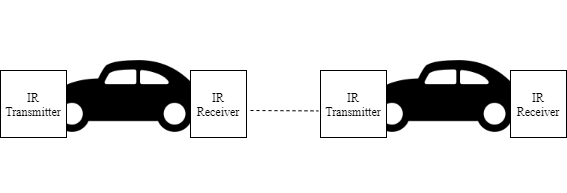
\includegraphics[width=0.9\textwidth]{Imgs/ir_diagram.png}
    \caption{\label{fig:frog}IR Receiver and Transmitter on RC Battle}
\end{figure}

\section{Project Requirements}
The requirements within the scope of the project are mentioned in this section. Project requirements are grouped under two separate headings as system requirements and functional requirements.

\subsection{Functional Requirements}
\begin{enumerate}
    \item Users should be able to connect to the RC car using remote control application which was developed within the scope of this project via Bluetooth.
    \item Users should be able to control the steering of the RC car using gyroscope and accelerometer of the phone.
    \item Users should be able to view the current steering angle on the user interface of the application.
    \item Users should be able to control the speed of the car by using slider on the user interface in both directions (forward and backward).
    \item Users should be able to view the current Li-Po battery charge percentage on the user interface of the application.
    \item Users should be able to trigger the IR transmitter of the RC car on the user interface of the application.
    \item After communication loss or non-healthy communication with the target RC Car, the RC car must stop all motors for safety with predefined threshold time.
    \item Users should be able to connect the online game server (database) on the user interface of the application.
    \item Users should be able to see the current score on the user interface of the application.
    \item A RC car should be able to hit the opponent RC car at least 1.5 meter away with IR transmitter of it.
\end{enumerate}

\subsection{System Requirements}
This section contains the system requirements of project, which are hardware requirements of the RC car robot and the remote controller application. Hardware and related electronic components discussed detailed in the section \ref{sec_hardware_design}\\

\begin{enumerate}
    \item STM32 Nucleo-64 development board.
    \item L298N Motor Driver, STMicroelectronics\texttrademark.
    \item HC05 Bluetooth\texttrademark\;module
    \item 5V 3A voltage regulator.
    \item 3S Li-Po Battery. Minimum capacity is 850 mAh.
    \item Bidirectional DC motor for accelerating.
    \item MG90s 50 Hz servo motor for steering. 
    \item IR receiver and IR transmitter module.
    \item Android\texttrademark\;smartphone with at least version Android 5.0.
\end{enumerate}

\begin{table}[!htbp]
    \centering
    \caption{\label{tab:widgets}An example table.}
    \begin{tabular}{l|r}
        Item & Quantity \\\hline
        Widgets & 45 \\
        Gadgets & 13
    \end{tabular}
\end{table}
\chapter{SYSTEM ARCHITECTURE} \label{chap_sys_architecture}
System architecture is explained and analyzed under three sub sections.
\begin{enumerate}
    \item Main overview of the system is explained in the Section \ref{sec_overview_sys_architecture}.
    \item Hardware design and architecture is explained in the Section \ref{sec_hardware_design}.
    \item Firmware design and architecture is explained in the Section \ref{sec_firmware_design}
    \item SİLİNECEK \cite{One, Two, Three}.
    
\end{enumerate}

\section{Overview of the System Architecture} \label{sec_overview_sys_architecture}

The system consist of paired RC car and Android phone. Android phone, which runs the remote control interface, connects the target RC car unit via Bluetooth communication and send / receive control packets over this channel. At server (database) side, each Android\texttrademark\;phone connects to the Firebase database in order to establish an online session for game. Figure \ref{fig:overview_architecture} shows the diagram of the main system architecture.

\begin{figure}[!htbp]
    \centering
    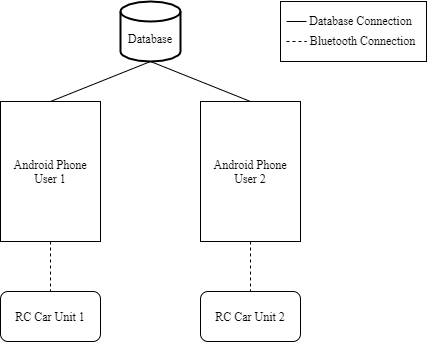
\includegraphics[width=0.8\textwidth]{Imgs/overview_of_sys.drawio.png}
    \caption{\label{fig:overview_architecture}Diagram of the Main System Architecture}
\end{figure}

\section{Hardware Design} \label{sec_hardware_design}

\subsection{Hardware Architecture} \label{sec_hardware_architecture}

Main hardware architecture and power / harness diagram is shown in Figure \ref{fig:hardware_architecture}. 

\begin{figure}[!htbp]
    \centering
    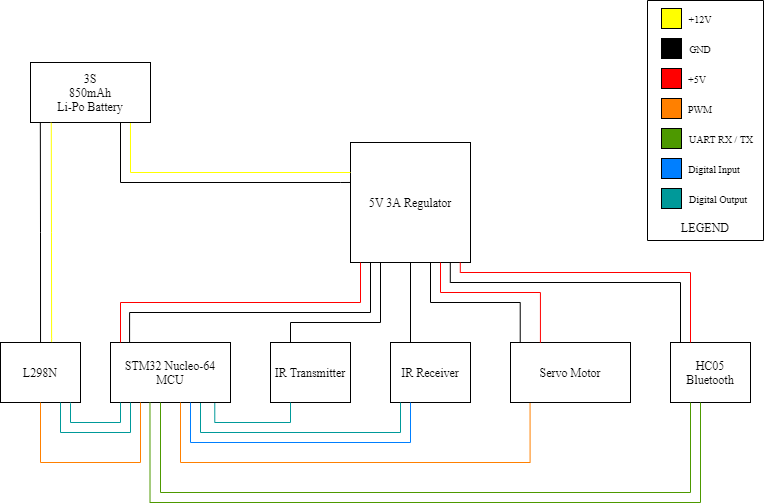
\includegraphics[width=1\textwidth]{Imgs/ana_devre_v3.png}
    \caption{\label{fig:hardware_architecture}Power / Harness Diagram of the Hardware}
\end{figure}

All system is powered from 3S 25C 850mAh Li-Po battery. This Li-Po battery can supply maximum current about 20A (C x mAh). This current capacity is enough for the supplying the system components. HC05 module, STM32 MCU and servo motor powered from the regulator output. This voltage regulator is a step down voltage regulator that decreases the voltage to 5V and supplies maximum 3A current.\\

L298N motor driver controlled by 3 input pins. 2 of these three input pins are controlling the direction of the DC motor. MCU writes digital output to these pins in order to change direction of the DC motor or completely stop the DC motor of the RC car unit. Other pin used for controlling the DC motor speed, by applying PWM signal to enable pin of the L298N motor driver. \\

Steering of the RC car controlled by the servo motor. This steering servo motor powered from voltage regulator 5V output and controlled from PWM signal that is generated by MCU of the RC car unit. \\

HC05 Bluetooth\texttrademark\;module connected to the UART pins of the MCU of the RC car unit. UART baud rate has been configured at 115200. HC05 RX pin is connected to the UART TX pin of the MCU, HC05 TX pin is connected to the UART RX pin of the MCU. By this way, MCU of the RC car unit communicate over the Bluetooth\texttrademark. \\

IR receiver is connected to the MCU of the RC car unit as a digital input in order to keep track of the hitting by the IR transmitter (led) coming from opponents RC car. IR transmitter (led) is connected to the MCU of the RC car unit as a digital input. By this way, IR transmitter (led) can be powered with GPIO pin whenever user wants.


% Hardware Components Part Start
\subsubsection{STM32 MCU}
The system uses STM32 Nucleo-64 development board as a MCU of the RC car unit. STM32 Nucleo-64 development board is based on processor Arm\textregistered\;Cortex\textregistered\;M4, has 32.768 kHz crystal oscillator,  has 11 timers: up to six 16-bit, two 32-bit timers up to 100 MHz, has 512 Kbytes of flash memory and 128 Kbytes of SRAM \cite{One}. This MCU provides necessary peripherals and clock speed for the RC car unit. This board has built-in ST link programming interface and driver which provides fast development without additional ST link device. The implementation of the hardware and firmware is not restricted with this development board, similar approach can be applied with any MCU that is based on Arm\textregistered\;Cortex\textregistered\;M4 family and that has sufficient number of timers, GPIOs and other essential peripherals. This development board is shown in Figure \ref{fig:nucleo64_board}.\\

\begin{figure}[!htbp]
    \centering
    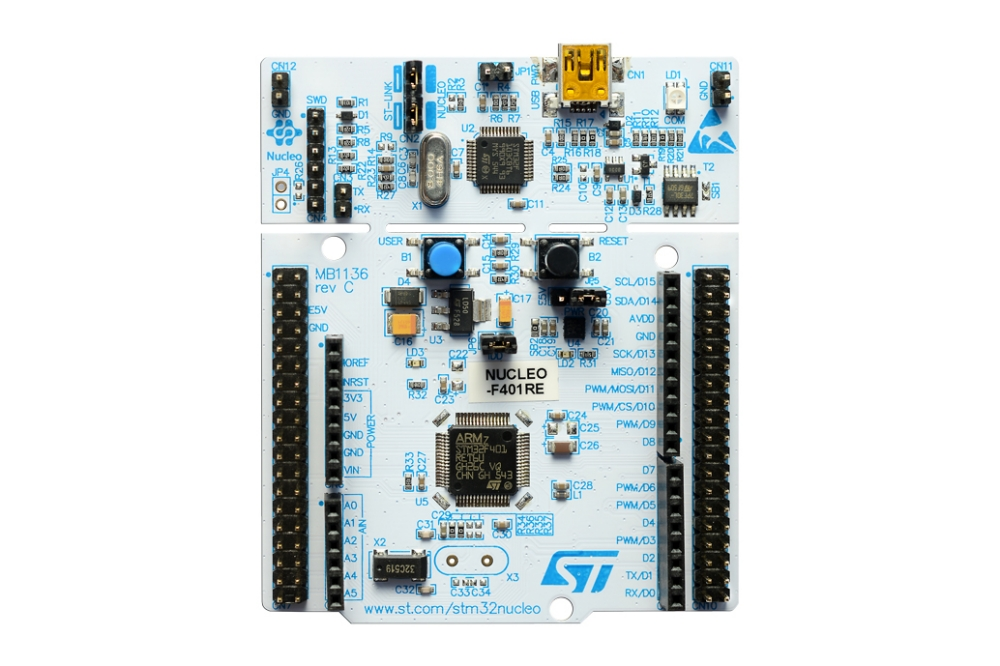
\includegraphics[width=0.9\textwidth]{Imgs/nucleo64.jpg}
    \caption{\label{fig:nucleo64_board}STM32 Nucleo-64 Development Board \cite{One}}
\end{figure}

\subsubsection{L298N DC Motor Driver}
STMicroelectronics\texttrademark\;L298N dual full bridge DC motor driver is used for driving the DC motor of the RC car unit. It is a high voltage, high current dual full-bridge driver designed to accept standard TTL logic levels and drive inductive loads such as relays, solenoids, DC and stepping motors. Two enable inputs are provided to enable or disable the device independently of the input signals. This enable inputs accepts PWM signals for driving motors with speed control. The L298N motor driver accepts 5-46V supply, provides maximum 2A DC current per channel \cite{Two}. According to these specifications and power ratings, this motor driver meets the requirements of the RC car unit. Motor driver PCB is show in Figure \ref{fig:l298n_pcb} .

\begin{figure}[!htbp]
    \centering
    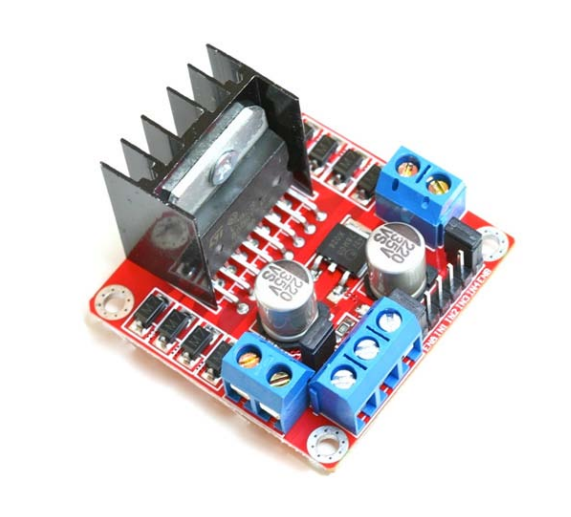
\includegraphics[width=0.5\textwidth]{Imgs/l298n.png}
    \caption{\label{fig:l298n_pcb}L298N Motor Driver PCB}
\end{figure}

\subsubsection{Servo Motor}
Servo motors have rapid acceleration and deceleration and provides high torques for many mechanic applications with allowing position control. High dynamic response and precision make them suitable for motion control applications and robotics. In the RC car unit, servo motor used for steering. Thus, precise steering control can be achieved.\\

In this project, TowerPro\texttrademark\; MG90S servo motor used. This servo motor works at 4.8V - 6V and has 1.8kg/cm stall torque. Maximum stall current consumption is about 1A \cite{Ref_servo_mg90s}. According to these running and power specifications, this servo motor meets the requirements of the RC car unit.


\subsubsection{Voltage Regulator}
LM2596 3A Step-Down Voltage Regulator is used for powering the system components which accept 5V for supply voltage. MCU, servo motor and HC05 Bluetooth\texttrademark\;module are powered from voltage regulator output. The LM2596 series of regulators are monolithic
integrated circuits that provide all the active functions for a step-down (buck) switching regulator, capable of driving a 3-A load with excellent line and load
regulation \cite{Three}. This voltage regulator supplies enough output current for powering the 5V components in the system.

\subsubsection{HC05 Bluetooth Module} \label{sec_hc05_module}
The Bluetooth\texttrademark\;wireless technology is designed as a short-range networking solution for personal, portable electronic devices and embedded systems. It overcomes the limitations of line of sight and one to one communication of its possible competitor Infra-Red(IR). It operates in the 2.4 GHz Industrial, Scientific and Medical (ISM) band at a maximum data rate of 720 Kbps \cite{Bluetooth_Overview}. \\

In RC Car Battle system, Bluetooth\texttrademark\;is used for communication between the RC car unit and the remote controller Android\texttrademark\;phone. HC05 Bluetooth\texttrademark\;module used for adding Bluetooth\texttrademark\;interface to the STM32 MCU of the system. HC05 module is Bluetooth SPP (Serial Port Protocol) module, designed for transparent wireless serial connection setup. It has integrated antenna and programmable UART interface. Baud rate, password, name of the can be configured over this UART interface in configuration mode \cite{HC05_datasheet}. This module allows MCU to communicate with Bluetooth\texttrademark\;over the UART interface. 115200 baud rate used for UART communication with the HC05 module. This module is shown in Figure \ref{fig:hc05_module}. \\ 

\begin{figure}[!htbp]
    \centering
    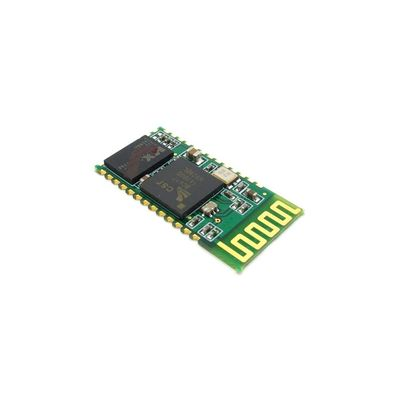
\includegraphics[width=0.5\textwidth]{Imgs/400px-HC-05.jpg}
    \caption{\label{fig:hc05_module}HC05 Bluetooth\texttrademark\; Module \cite{HC05_datasheet}}
\end{figure}

\subsubsection{IR Transmitter and Receiver Module}
The RC car units simulates the shooting and hitting by IR transmitter (IR Led) and IR receiver module which. Keyestudio\texttrademark\;infrared obstacle avoidance sensor (IR-08H) used for achieving this functionality. Main purpose of this module is estimating distance by using IR led and IR receiver for obstacle avoidance applications on robotic systems. It has a pair of infrared transmitting and receiving tube. When infrared ray launched by the transmitting tube encounters an obstacle (its reflector), the infrared ray is reflected to the receiving tube, and the indicator will light up; the signal output interface outputs digital signal. This module works at DC 3.3V-5V voltage values. The logic level 3.3V and power consumption ratings are compatible with the MCU of the RC car unit.\\

IR transmitter and receiver module has been modified for this project. A RC car unit has two of this IR module, one for transmitter which is on front side of the RC car, one for receiving IR light which is on back side of the RC car. IR receiver part removed from the transmitter IR module. IR transmitter (led) part removed from the receiver IR module. 

% Hardware Components Part End

\subsection{RC Car Control Unit}
In this project, custom RC car control unit has been designed on PCB. The designed and developed multi-layered PCB gathers system components under a single circuit. The PCB contains female and male headers for system components. The motivation behind the design and produce PCB is avoid short circuit and loose electrical connections. The RC car control unit provides robust connection between system components and electronic modules. The designed PCB contains the following system component connections :
\begin{enumerate}
    \item Servo and DC motor male header pins.
    \item HC05 Bluetooth\texttrademark\;female header pins.
    \item STM32 MCU female header pins.
    \item Voltage regulator pad connections.
    \item L298N motor driver pad connections.
    \item Voltage divider circuit, resistor connections.
    \item Input power male header pins.
    \item Jumper for selecting the Li-Po battery ADC input with male headers.
    \item UART male header pins for debugging.
\end{enumerate}


\begin{figure}[!htbp]
    \centering
    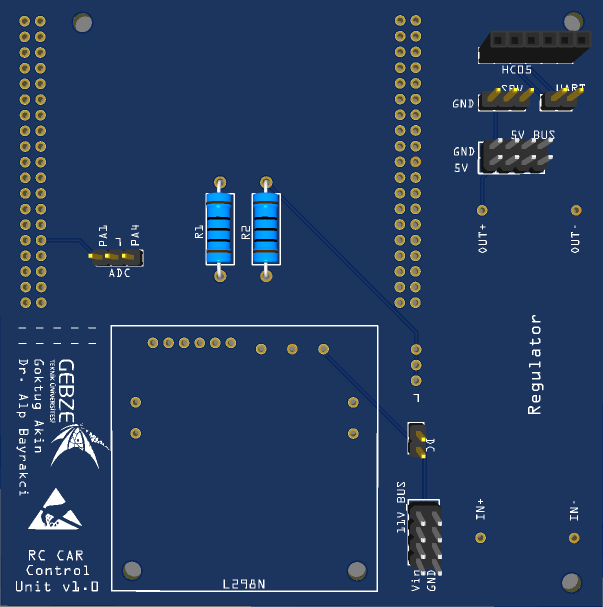
\includegraphics[width=0.75\textwidth]{Imgs/pcb.png}
    \caption{\label{fig:custom_pcb}Design View of RC Car Control Unit PCB}
\end{figure}

Manufactured, real version of the control unit PCB is shown in Figure .


\section{Firmware} \label{sec_firmware_design}

\subsection{Bidirectional Reliable Bluetooth Communication} \label{sec_bluetooth_comm}

Communication with the controller smartphone and the RC car unit provided via Bluetooth\texttrademark.\;Hardware details of the Bluetooth\texttrademark\;explained in the Section \ref{sec_hc05_module}. This section explains the implementation details of the bidirectional Bluetooth\texttrademark\; communication.

\subsubsection{UART RX Registers} \label{sec_receive_rc_command}

The remote controller smartphone sends RC command to the target RC car unit at 10 HZ. HC05 module receives the incoming data from the controller smartphone, and sends these incoming data to the UART peripheral of MCU of the RC car unit. This communication runs at 115200 baud-rate. \\

The UART unit of the STM32 MCU generates IRQ when new data available on the UART line. Custom ISR has been implemented for catching and handling the interrupts. The UART interrupts used for efficient communication instead of polling method in order to avoid consuming unnecessary cycles. UART line is authorized in the NVIC unit of the MCU for an interrupt to occur from the UART unit of the MCU. \\

To able to enable the read interrupts from the UART unit, RXNEIE (RX not empty interrupt enabled) bit of the CR1 (Control Register 1) has been set to 1. After this configuration, when there is a new data to be read on the UART line, an interrupt will be generated from the UART unit. This control register is shown in Figure \ref{fig:uart_cr_register}. RXNEIE bit of the register highlighted in yellow.

\begin{figure}[!htbp]
    \centering
    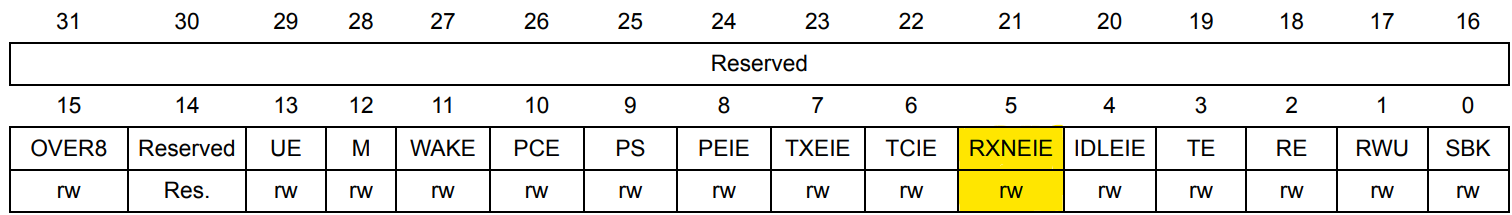
\includegraphics[width=1\textwidth]{Imgs/cr_register.png}
    \caption{\label{fig:uart_cr_register}UART Control Register 1 of the MCU (1) \cite{Ref_stm32_um}}
\end{figure}

When there is new data on the UART line, RXNE (RX not empty) bit of the status register (SR) of the UART unit being set to 1 by hardware. This bit is cleared by a read to the DR register of UART which contains the incoming data (byte). This status register is shown in Figure \ref{fig:uart_sr_register}. RXNE bit of the register highlighted in yellow.

\begin{figure}[!htbp]
    \centering
    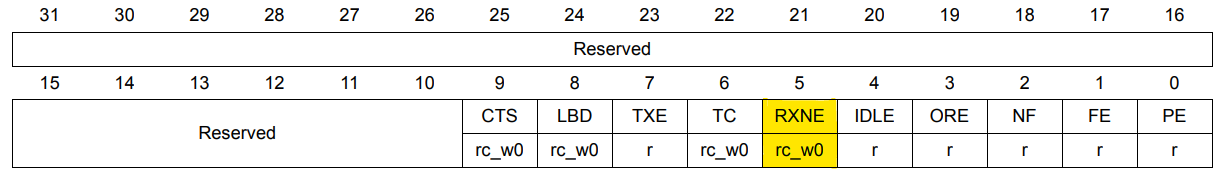
\includegraphics[width=1\textwidth]{Imgs/sr_register.png}
    \caption{\label{fig:uart_sr_register}UART Status Register of the MCU (1) \cite{Ref_stm32_um}}
\end{figure}


\subsubsection{UART TX Registers}
\label{sec_transmit_rc_info}

The RC car unit sends RC car information packet to the controller smartphone at 1 HZ. The MCU sends the data over the UART line, which is connected to the HC05 module. The information packet contains the version of the firmware, Li-Po battery percentage and hit counter. The controller smartphone receives these information packets in order to view in the user interface and send the related information to the database (game server).

The UART unit of the STM32 MCU generates IRQ when TX sending buffer is empty for sending new data. Custom ISR has been implemented for catching and handling the interrupts. When the IRQ is triggered, the data register of the UART unit is filling by the byte which is next in the ISR.

To able to enable the write available interrupts for UART unit, TXEIE (TX empty interrupt enabled) bit of the CR1 (Control Register 1) has been set to 1. After this configuration, when TX buffer of the UART unit is empty, an IRQ will be generated from the UART unit. The control register is shown in Figure \ref{fig:uart_cr_tx_register}. TXEIE bit of the register highlighted in yellow.

\begin{figure}[!htbp]
    \centering
    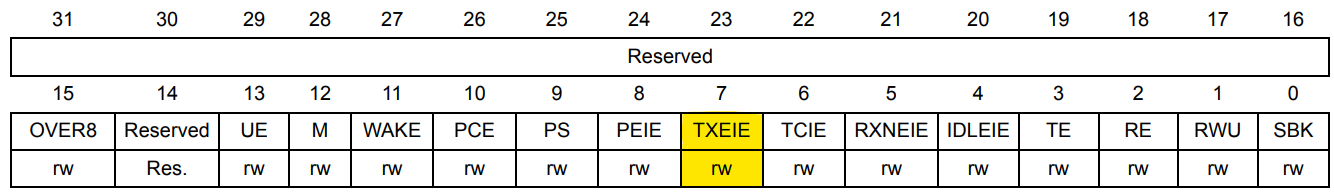
\includegraphics[width=1\textwidth]{Imgs/cr_tx_register.png}
    \caption{\label{fig:uart_cr_tx_register}UART Control Register 1 of the MCU (2) \cite{Ref_stm32_um}}
\end{figure}

When TX buffer of the UART unit is empty, TXE bit of the status register (SR) of the UART unit being set to 1 by hardware. This bit is cleared by write to the DR register of the UART unit, which contains the data (byte) to be sent to the TX buffer of the UART unit. This status register is shown in Figure \ref{fig:uart_sr_tx_register}. TXE bit of the register highlighted in yellow.

\begin{figure}[!htbp]
    \centering
    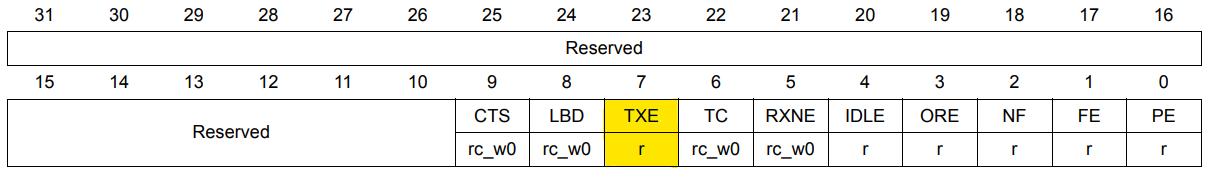
\includegraphics[width=1\textwidth]{Imgs/sr_tx_register.png}
    \caption{\label{fig:uart_sr_tx_register}UART Status Register of the MCU (2) \cite{Ref_stm32_um}}
\end{figure}


\subsubsection{UART Circular Buffer Implementation}
\label{sec_uart_circular_buff}

A circular buffer is a FIFO data structure that considers memory to be managed circularly; that is, the read/write indices loop back to 0 after it reaches the buffer length. Circular buffer has a fixed size allocated once at the system run-time. Tail and head pointers used to indicate where to read or write to the buffer mechanism. Each time a new data sample is added (write) into the buffer, the head pointer is incremented and when the data is being read the tail pointer is incremented \cite{Ref_circ-buffer} \cite{Ref_circ_buffer_paper}. In this mechanism, producer consumer paradigm can be easily utilized over the buffer.

The Algorithm \ref{isr_rx_algorithm} shows the pseudo code of the ISR of the UART unit.

\begin{algorithm}
\caption{ISR of UART unit}
\label{isr_rx_algorithm}
    \begin{algorithmic}
    \If{RXNE bit of the SR is 1 \textbf{AND} RXNEIE bit of the CR1 is 1}
        \State read byte from UART->DR, push into circular buffer.
        \State increment head position of the circular buffer.
    \EndIf
    \If{TXE bit of the SR is 1 \textbf{AND} TXEIE bit of the CR1 is 1}
        \If{tail position is head position}
            \State set TXEIE 0 for disabling TXE interrupts.
        \ElsIf{tail position is not head position}
            \State read byte from the circular buffer, push into USART->DR.
            \State increment tail position of the circular buffer.
        \EndIf
    \EndIf
    \end{algorithmic}
\end{algorithm}




\subsection{Controlling Motors} \label{sec_controlling_motors}

\subsection{IR Receiver and IR Transmitter} \label{sec_ir_rx_tx}

\subsection{Reading Li-Po Battery Voltage} \label{sec_read_lipo_voltage}

\subsection{Main Overview of the System Components} \label{main_system_components}

\section{Remote Controller Application} \label{sec_remote_app}

\subsection{User Interface} \label{sec_user_interface}

\subsection{RC Car Communication} \label{sec_rc_comm}

\subsection{Database Connection} \label{sec_db_connection}



\begin{comment}
% Below are comments, just for source..
\begin{algorithm}
\caption{ISR of UART line for RX interrupts}
\label{isr_rx_algorithm}
\begin{algorithmic}
\Require $n \geq 0$ % i.e. input
\Ensure $y = x^n$  % i.e. output
\State $y \gets 1$
\State $X \gets x$
\State $N \gets n$
\While{$N \neq 0$}
\If{$N$ is even}
    \State $X \gets X \times X$
    \State $N \gets \frac{N}{2}$  \Comment{This is a comment}
\ElsIf{$N$ is odd}
    \State $y \gets y \times X$
    \State $N \gets N - 1$
\EndIf
\EndWhile
\end{algorithmic}
\end{algorithm}
    Ut enim ad minima veniam, quis nostrum exercitationem ullam corporis suscipit laboriosam, nisi ut aliquid ex ea commodi consequatur? Quis autem vel eum iure reprehenderit qui in ea voluptate velit esse quam nihil molestiae consequatur, vel illum qui dolorem eum fugiat quo voluptas nulla pariatur? \ref{tab:widgetss}

    \begin{table}[!htbp]
    \centering
    \caption{\label{tab:widgetss}Comparison of percentages.}
    \begin{tabular}{c|cc|cc}
    \hline
    Mode &  \multicolumn{2}{c}{Var} & \multicolumn{2}{c}{Cum}\\ 
    \hline
    1   &  17.5 & 19.1   & 17.5  & 19.1\\
    2   &  11.8 & 12.7   & 29.3  & 31.9\\
    3   &  6.6  &  5.6   & 35.9  & 37.4\\
    \end{tabular}
    \end{table}
    
    \begin{enumerate}
    \item first,
    \item second.
    \end{enumerate}
    \dots and bullet points \dots
    \begin{itemize}
    \item one bullet,
    \item two bullets.
    \end{itemize}
    
    Let $X_1, X_2, \ldots, X_n$ be a sequence of independent and identically distributed random variables with $\text{E}[X_i] = \mu$ and $\text{Var}[X_i] = \sigma^2 < \infty$, and let
    \[S_n = \frac{X_1 + X_2 + \cdots + X_n}{n}
          = \frac{1}{n}\sum_{i}^{n} X_i\]
    denote their mean. Then as $n$ approaches infinity, the random variables $\sqrt{n}(S_n - \mu)$ converge in distribution to a normal $\mathcal{N}(0, \sigma^2)$.
    
    \begin{quote}
        At vero eos et accusamus et iusto odio dignissimos ducimus qui blanditiis praesentium voluptatum deleniti atque corrupti quos dolores et quas molestias excepturi sint occaecati cupiditate non provident, similique sunt in culpa qui officia deserunt mollitia animi, id est laborum et dolorum fuga.
    \end{quote}
\end{comment}
\chapter{Conclusions}
In this study, the RC car battle framework which provides an online game environment to users has been developed. The main motivation of this study is combining the capabilities of the smartphones and embedded devices for creating a framework which provides a multiplayer shooter game over the robot cars. Users play an online shooter game by their remote controller smartphone of the target RC car device, instead playing in a virtual environment.

Next version of this study can provide following functionalities for better game environment and user experience, since the technology behind the MCU and the smartphone of the system supports these features:

\begin{itemize}
    \item Adding GPS to the RC car device in order to view the location of the car in the user interface while playing the shooter game.
    \item Adding options for steering control which are controlling with a button or a virtual steering wheel.
\end{itemize}




% DON'T INPUT FILES AFTER HERE
\begin{outertitles}
\clearpage
\setlength{\emergencystretch}{1em}
\printbibliography
\addtocontents{toc}{\protect\vspace{18pt}}
\addcontentsline{toc}{chapter}{Bibliography}
%% If you don't want a CV or appendices add a % at the beginning of the relevant line
%\chapter*{CV}
\addcontentsline{toc}{chapter}{CV}

%% Edit below this line
XXX.



%% Until here
\clearpage
%\chapter*{Appendices}
\addcontentsline{toc}{chapter}{Appendices}

\section*{Appendix 1: Some publications}

No one significant, in AAA.

\section*{Appendix 2: Some explanation}

None needed mate!
\end{outertitles}
\end{document}